\section{Performance Evaluation}
\label{chap:eval}

In this chapter we discuss the performance results that we achieved using \cphash{} and \cpserver{}. In the following sections we 
first discuss our alternative implementations that were developed for comparative benchmarking. Then we present our evaluation of the scalability 
and performance of \cphash{}. Finally we provide the benchmark results for \cpserver{}

\subsection{Alternative Hash Table and Key/Value Cache Server Implementations using Locks}

To evaluate the performance and scalability of \cphash{}, we created an alternative implementation
of the hash table that does not use computation migration. This version is implemented in a traditional shared memory 
style with scalable fine-grained locks. In this alternative implementation, each partition is protected by
a lock and there are no server threads. The client threads process queries by first acquiring the lock for
the appropriate partition, then performing the query, updating the LRU list and, finally, releasing the lock. We call this implementation \lockhash{}.
We use this alternative implementation for comparison with \cphash{} to show that computation migration provides much
better scalability and performance than having scalable locks.

In addition to developing the alternative hash table implementation we also developed an alternative key/value cache server implementation
that uses \lockhash{} as its hash table instead of \cphash{}. We call this alternative server implementation \lockserver{}.

\subsection{Hash Table Performance}

We created a simple benchmark that tests various aspects of the hash table implementations. The benchmark generates random queries and
performs them on the hash table. A single query can be either a LOOKUP or an INSERT operation. The INSERT operation consists of 
inserting key/value pairs such that the key is a random number and the value is the same as the key (8 bytes). 

The benchmark can be configured using several parameters:
\begin{itemize}
\item Number of Partitions (i.e. number of server threads)
\item Number of Client Threads/Cores
\item Size of Batch
\item Maximum cache size in bytes
\item Hash INSERT ratio over total number of queries
\item Maximum Value of Hash Key
\item Number of iterations
\end{itemize}

We use a 48 core AMD64 machine for our testing. This machine has eight six-core processors of type AMD Opteron(tm) 8431. Each core has
a 512KB L2 cache and each six-core processor has a unified 6MB L3 cache.

\subsubsection{Scalability}

The first experiment evaluated the scalability of the \cphash{} implementation. We ran our benchmark with an equal number of server 
and client threads varying from 3 to 24 (i.e. using 6 to 48 cores $-$ half of the cores for the server threads, and the other half for the 
client threads), with a total hash table size of 10 MB, with 30\% INSERT ratio, with keys ranging from 0..$2^{17}$, and for $10^{8}$ iterations. 
We also ran our \lockhash{} implementation with the same exact parameters using 6 to 48 cores. Figure \ref{fig:scale10mb} shows the 
throughput per core for \cphash{} and \lockhash{} on a 10 MB hash table.

We also ran the same tests but with a hash table size of 1 GB with keys ranging from 0..$2^{24}$. In this case, we ran the benchmark for $10^{9}$ iterations to make
sure that the hash table was full for most of the iterations. Figure \ref{fig:scale1gb} shows the throughput per core for \cphash{} and \lockhash{} on the
1 GB hash table.

\begin{figure}[!ht]
  \centering
  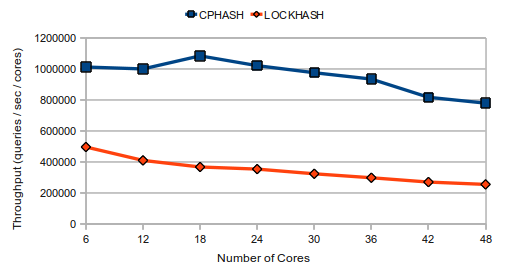
\includegraphics[width=0.8\linewidth]{figs/scale10mb.png}
  \caption{Throughput per core on 10 MB hash table}
  \label{fig:scale10mb}
\end{figure}
    
\begin{figure}[!ht]
  \centering
  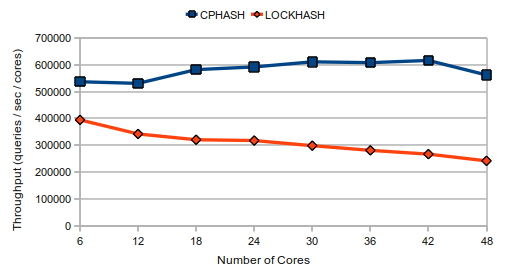
\includegraphics[width=0.8\linewidth]{figs/scale1gb.png}
  \caption{Throughput per core on 1 GB hash table}
  \label{fig:scale1gb}
\end{figure}

These graphs show that the \cphash{} implementation has better scalability than the \lockhash{} implementation. However, we do not 
get a complete linear speedup for small hash tables. The reason for this is the message passing overhead. This overhead is more significant for smaller 
hash tables since most other memory operations are cache hits, thus, message passing takes a significant percentage of the total computation time. On
the other hand \cphash{} achieves great scalability for larger hash table. It achieves a super-linear speedup in Figure \ref{fig:scale1gb} due to the fact that
as the number of cores increases, its combined L2 and L3 cache space is larger, resulting in fewer cache misses per query and higher throughput per core. 

As the number of cores increases, message passing becomes more expensive due to the hardware architecture. If the cores are physically farther apart from each 
other, the message passing cache miss will take longer to complete. To prove this hypothesis we ran our benchmark with a small empty hash table, and no INSERTs. 
In this scenario message passing takes most of the computation time. Figure \ref{fig:scalemp} shows the declining throughput as the number of cores increases.

\begin{figure}[!ht]
  \centering
  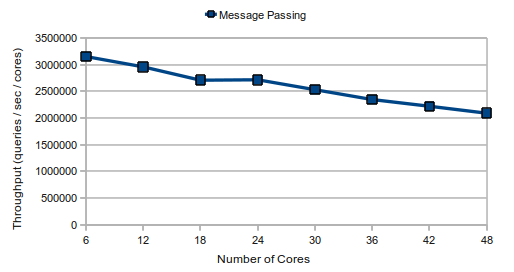
\includegraphics[width=0.8\linewidth]{figs/scalemp.png}
  \caption{Message Passing Throughput per core}
  \label{fig:scalemp}
\end{figure}

\subsubsection{Performance}

Figure \ref{fig:cphashspeedup} shows the throughput gains of \cphash{} compared to the \lockhash{} implementation for the tests described in 
the previous section, as well as for a 40 MB hash table.

\begin{figure}[!ht]
  \centering
  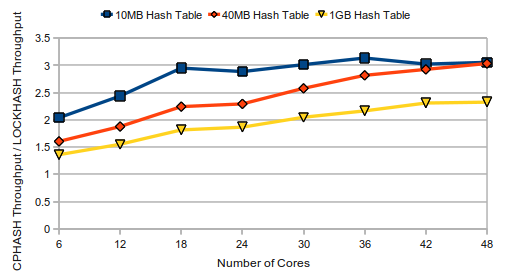
\includegraphics[width=0.8\linewidth]{figs/cphashspeedup.png}
  \caption{\cphash{} throughput vs \lockhash{} throughput}
  \label{fig:cphashspeedup}
\end{figure}

The performance of \cphash{} does not depend on the actual size of the hash table but rather on the number of elements in it. This is because the server 
threads never access or modify the values in the hash table but just the meta data (buckets, chain lists, LRU list etc). In our benchmarks the value of 
each element has the same size (8 bytes), therefore, the number of elements in the hash table is proportional to the size of the table.

The results shown in Figure \ref{fig:cphashspeedup} are consistent with the scalability graphs. \cphash{}'s throughput per core decreases after all 
the hash table meta data fits in the combined hardware caches of the server cores. This is the main reason why we do not see any increase in throughput ratio after 
the number of cores reaches 18, for 10 MB hash table. The current bottleneck for scalability on small hash tables is the \cphash{}'s message passing implementation.

\subsubsection{Summary}

The benchmark results show that \cphash{} is scalable and provides increased throughput, especially when the hash table meta data fits in the server cores'
combined hardware caches. When the hash table meta data is much larger than the combined caches, \cphash{} still provides some benefits through batching and caching 
the common partition data (such as an LRU list).

There is another scenario when \cphash{} is beneficial for large hash tables. Even though most of the time the load on the hash table may not be significant
and the performance is acceptable, there might be certain peak times when a specific small subset of the hash table experiences heavy load (i.e. most of the queries involve 
operations on keys in that subset). If this subset is small enough so that its meta data fits into the combined caches of server cores, then the \cphash{} 
implementation can significantly improve performance.

\subsection{Key/Value Cache Server Performance}
\label{sec:mcserverbench} 

We tested the performance of our \cpserver{} against the \lockserver{} and \memcached{}. For these benchmarks we used a 16 core AMD64 machine as 
our server. This 16 core machine has four quad-core processors of type AMD Opteron(tm) 8350. Each core has a 512KB L2 cache, and each quad-core processor has a 
unified 4MB L3 cache. 

We developed a benchmark client for the Key/Value Cache Server. We used our 48 core AMD64 machine as a load generator to run the benchmark clients. 
The load generator machine and the server machine were connected with 10 GBit Ethernet network. We made sure in our benchmarks that we were generating enough load to 
bottleneck the servers, so that the speed of a single benchmark client would not affect the performance. We also made sure that the servers were CPU and Memory 
bottlenecked and that the network was not the limiting factor. To achieve this, in addition to having 10GBit Ethernet network, we used a 
patch for the Linux kernel network driver \cite{mosbench} to make it more scalable.

The benchmark client has following configuration parameters:
\begin{itemize}
\item Size of Batch
\item Hash INSERT ratio over total number of queries
\item Maximum Value of Hash Key
\item Size range for Hash Value
\item Number of iterations
\end{itemize}

First we compared the performance of \cpserver{} to \lockserver{}. We ran the servers with a 16 GB hash table. Before starting any benchmarking we 
made sure to completely fill up the hash table with random data. We set the batch size to 1000, and the size range for the hash values to 8$-$128 bytes. We run our tests 
for 80 million iterations.

We varied the INSERT ratio from 0\% to 100\% with 20\% steps. We tried three different Hash Key ranges: 0..2$^{16}$, 0..2$^{23}$, and 0..2$^{28}$. A 16 GB hash table
can hold around 160 million elements when the size of values are 8 to 128 bytes. Therefore when running with Hash Key ranges of 0..2$^{16}$ or 0..2$^{23}$, the hit rate 
is 100\%. On the other hand when running with a key range of 0..2$^{28}$ it is around 60\%-70\%. Figure \ref{fig:cpserverspeedup} shows the throughput gains of 
\cpserver{} compared to \lockserver{}.

\begin{figure}[!ht]
  \centering
  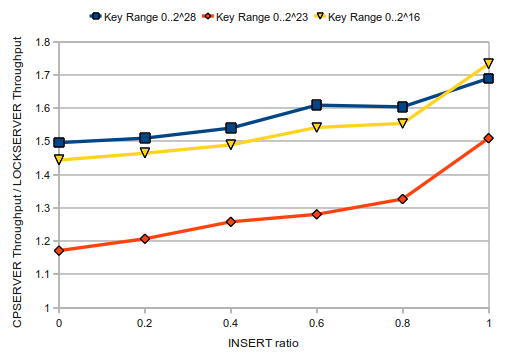
\includegraphics[width=0.8\linewidth]{figs/cpserverspeedup.png}
  \caption{\cpserver{} throughput vs \lockserver{} throughput}
  \label{fig:cpserverspeedup}
\end{figure}

There are four major factors that affect the speedup: Hit Rate, INSERT ratio, size of the hash table (or the range of hash keys), and the size of the hash values. 
Smaller Hit Rate and higher INSERT ratio result in larger speedups for \cpserver{}. This is because hash INSERTs are silent (i.e. the server does not return 
any response for them), and LOOKUP misses just return a single 32 bit value. Thus, for hash INSERTs and LOOKUP misses, most of the computation time for a query is taken by 
the hash table operation and not by the writes to the TCP connection buffer. 

Larger hash values work against the \cpserver{} implementation. If hash values are large most of the computation time during LOOKUP query hits is spent on 
writing back the value to the TCP buffer. For very large hash values the \lockserver{} can outperform the \cpserver{} since it has more threads 
writing to the buffers which results in better performance.

The size of the hash table or the range of the hash keys affects performance since, as we showed in the previous section, if the meta data of all the elements 
that are accessed can fit into the combined caches of the server cores, the hash operations in \cphash{} will be faster than in \lockhash{}.

Figure \ref{fig:cpserverspeedup} confirms our hypotheses. With key ranges of 0..2$^{16}$ or 0..2$^{23}$ the hit rate is 100\%; however, the meta data of 
2$^{16}$ elements fits into the combined caches of 8 server cores, resulting in a higher speedup. For the key range of 0..2$^{28}$ the hit rate is around 65\%; 
therefore, there is less time spent on writing buffers and more time spent on the actual hash operations resulting in a higher overall speedup.

\subsubsection{Performance against \memcached{}}
We compared the performance of \cpserver{} to \memcached{}. We ran 16 \memcached{} servers with 1 GB size limit each (16 GB total) on our server machine.
We extended the benchmark client with the \texttt{libmemcached} library \cite{libmemcached} to run same the benchmarks for \memcached{} as the ones described in
the previous section. However, since the \memcached{} protocol supports batching only for LOOKUPs, we performed the tests with only LOOKUP operations. As in previous 
test runs we made sure to fill up hash table server with some random elements before running any benchmarks. 

We ran tests with two different hash value size ranges: 8 to 128 bytes and 8 to 512 bytes. 
Tables \ref{table:memcachedspeedup0} and \ref{table:memcachedspeedup1}, show the results for the two scenarios described.

Since the \memcached{} protocol has a higher overhead per each request and response sent, we also compared the performance of \cpserver{} with hash value 
ranges of 72 to 192 bytes to \memcached{} with value ranges of 8 to 128 bytes. The results for this test run are provided in Table \ref{table:memcachedspeedup2}.

The tables give total running times for \cpserver{} and \memcached{} (in seconds) and also provide the average hit rate per each LOOKUP operation.
Figure \ref{fig:cpserverspeedup2} shows the throughput gains of \cpserver{} compared to \memcached{} based on values provided in the tables. 

\begin{table}[!ht]
\centering
\caption{Speedup with hash value size range of 8 to 128 bytes} 
\label{table:memcachedspeedup0}
\begin{tabular}{ | c | c | c | c | c | }
  \hline
  Key Range & \cpserver{} & \memcached{} & Speedup & Hit rates \\
  \hline
  0..2$^{28}$ & 13.563 & 35.618 & 2.626 & 0.655 vs 0.817 \\
  0..2$^{23}$ & 22.102 & 39.741 & 1.798 & 1.0 vs 1.0     \\
  0..2$^{16}$ & 16.719 & 39.512 & 2.363 & 1.0 vs 1.0     \\
  \hline
\end{tabular}
\end{table}

\begin{table}[!ht]
\centering
\caption{Speedup with hash value size range of 8 to 512 bytes} 
\label{table:memcachedspeedup1}
\begin{tabular}{ | c | c | c | c | c | }
  \hline
  Key Range & \cpserver{} & \memcached{} & Speedup & Hit rates \\
  \hline
  0..2$^{28}$ & 27.587 & 41.753 & 1.514 & 0.688 vs 0.750 \\
  0..2$^{23}$ & 43.532 & 46.251 & 1.062 & 1.0 vs 1.0     \\
  0..2$^{16}$ & 39.845 & 46.388 & 1.164 & 1.0 vs 1.0     \\
  \hline
\end{tabular}
\end{table}

\begin{table}[!ht]
\centering
\caption{Speedup with larger hash value size range for \cpserver{}} 
\label{table:memcachedspeedup2}
\begin{tabular}{ | c | c | c | c | c | }
  \hline
  Key Range & \cpserver{} & \memcached{} & Speedup & Hit rates \\
  \hline
  0..2$^{23}$ & 23.240 & 39.741 & 1.710 & 1.0 vs 1.0   \\
  0..2$^{16}$ & 19.329 & 39.512 & 2.044 & 1.0 vs 1.0   \\
  \hline
\end{tabular}
\end{table}

\begin{figure}[!ht]
  \centering
  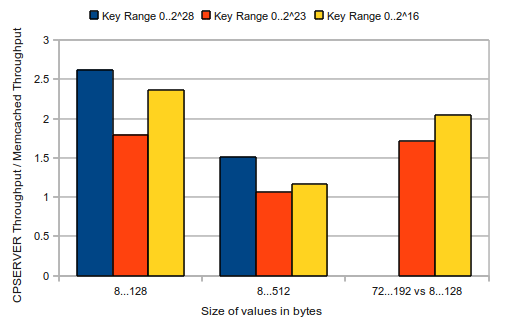
\includegraphics[width=0.8\linewidth]{figs/cpserverspeedup2.png}
  \caption{\cpserver{} throughput vs \memcached{} throughput}
  \label{fig:cpserverspeedup2}
\end{figure}

The results achieved are similar to the results achieved against \lockserver{}. Smaller hit rate, smaller values and smaller key range all benefit the
\cpserver{} implementation for the same reasons as described in the previous section. On the other hand, as can be noticed in the second row of Table 
\ref{table:memcachedspeedup1}, when the hit rate is 100\% and the value range is 8 to 512 bytes, \cpserver{} has almost no advantage over \memcached{},
especially when the size of hash table is much larger than size of combined L2 and L3 caches of all the server cores.

The results indicate that \cpserver{} outperforms \memcached{} in several specific scenarios; however, a performance evaluation with a load specific to a 
real-world application or web-server is needed for a more comprehensive comparison of the two server implementations. 

